\chapter{Introduction}
Lipids are amphiphilic molecules, consisting of a hydrophilic headgroup
and hydrophobic chains. There are various kinds of lipids. These can be 
categorized in terms of headgroup, chain length, and chain saturation.

In water lipids self-assemble into lipid bilayes to shield their hydrophobic 
cores. Lipid bilayers are the building blocks of cell membranes. Lipid bilayers 
display a wide variety of thermodynamic phases
as a function of temperature and hydration. Figure~\ref{fig:phase_diagram}
shows a phase diagram of dimyristoylphosphatidylcholines (DMPC).
At full hydration, a lamellar phase coexists with excess water.
PC lipids constitute a substantial fraction of cell membranes
and have been studied for many decades.
In the high temperature, fluid L$_\alpha$ phase, the hydrocarbon chains 
are conformationally disordered, and intra-membrane molecular correlations 
are liquid-like \cite{ref:Fahey78} (Fig.~\ref{fig:various_phases}).
In the low temperature, gel L$_{\beta'}$
phase, hydrocarbon chains are stiff and titled with respect to the membrane
normal \cite{ref:Tardieu73}, and are organized in a either hexagonal 
or orthorhombic lattice. 
The L$_{\beta'}$ is further categorized into three phases according to the 
chain tilt direction \cite{ref:Smith88}. 
In the L$_{\beta\text{I}}$ phase, chains are titled toward the 
nearest neighbor as shown in Fig.~\ref{fig:gel_phase_packing}, and
in the \LbetaF\ phase, chains are titled toward the next-next nearest neighbor.
In the \LbetaL\ phase, chains are tilted toward an intermediate direction.

\begin{figure}[htbp]
  \centering
  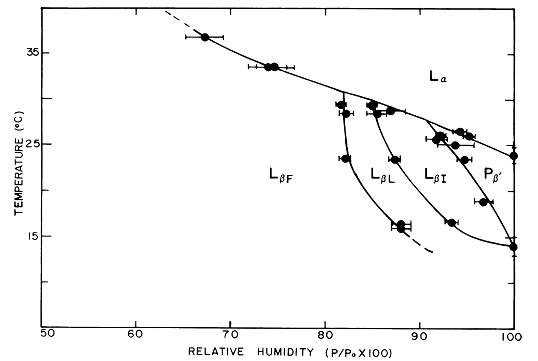
\includegraphics[width=0.9\textwidth]{figures/ripple/smith_phase_diagram}
  \caption{Experimental phase diagram of DMPC from Ref.~\cite{ref:Smith88}.
  \LbetaI, \LbetaL, and \LbetaF\ belong to the gel L$_{\beta'}$ phase. P$_{\beta'}$ is 
  the ripple phase and L$_\alpha$ is the fluid phase.}
  \label{fig:phase_diagram}
\end{figure}

\begin{figure}[htbp]
  \centering
  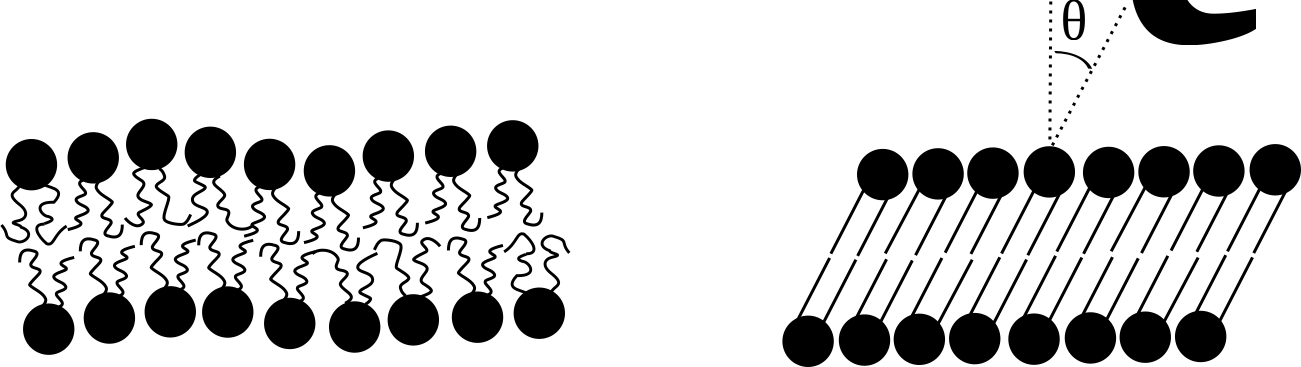
\includegraphics[width=0.9\textwidth]{figures/ripple/various_phases}
  \caption[]{Schematics of the structure of fluid L$_\alpha$ phase (left) and 
  gel L$_{\beta'}$ phase (right). Black solid circles are lipid headgroups 
  and solid lines are lipid chains. $\theta_t$ is the chain tilt angle.}
  \label{fig:various_phases}
\end{figure}

\begin{figure}[htbp]
  \centering
  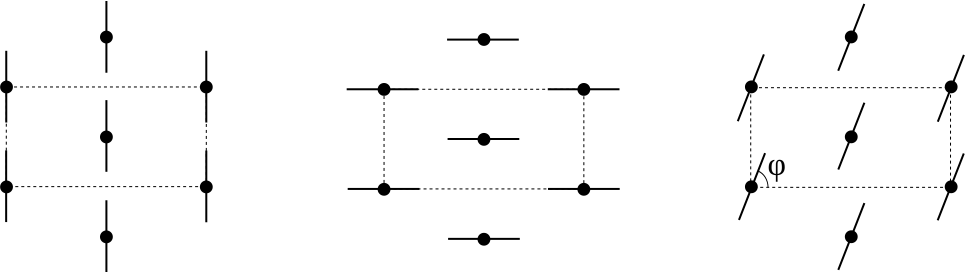
\includegraphics[width=0.9\textwidth]{figures/ripple/gel_phase_packing}
  \caption{Chain tilt direction in \LbetaI\ (left), \LbetaF\ (middle), and
  \LbetaL\ (right) phases. Black dots are orthorhombic lattice points.
  Unit cells are shown in dashed lines.
  Chains are drawn as solid lines. Chains are tilted toward the
  nearest neighbor in \LbetaI\ phase with $\phi=\pi/2$. 
  In \LbetaF\ phase, they are titled toward the next-next nearest neighbor
  ($\phi=0$). In \LbetaL\ phase, $\phi$ can be anywhere between 0 and $\pi/2$.}
  \label{fig:gel_phase_packing}
\end{figure}

Between the fluid and gel phases appears a height modulated phase where
bilayers are no longer flat (Fig.~\ref{fig:various_phases}). 
The low angle diffraction pattern of this phase conforms to the symmetry
of a two dimensional monoclinic lattice. This phase was termed P$_\beta'$ 
and is commonly
called the ripple phase. The P$_{\beta'}$--L$_{\beta'}$ transition is often
called the pre-transition.
The topography of the membrane ripples has been directly
visualized by freeze fracture electron microscopy experiments 
\cite{ref:Luna77,ref:Copeland80,ref:Ruppel83,ref:Zasadzinski87,ref:Zasadzinski88}.
The wavelength of the modulation is about 140 \AA\ for 
dimyristoylphosphatidylcholine (DMPC),
which has 14 carbons in the hydrocarbon chains \cite{ref:Wack89}.
There has been evidence that molecular conformation in the ripple phase is not 
unique. NMR signals in the ripple phase \cite{ref:Wittebort81} were consistent
with a superposition of signals observed in the fluid and gel phases.
Lateral diffusion measurements found two distinct populations,
with diffusion coefficients characteristic of fluid and gel phases
\cite{ref:Schneider83}. 



In this thesis, we forcus on the fluid and ripple phases. In the former phase,
we investigated the interaction of Tat peptide with lipid bilayers. 
This study is discussed in chapter 2.
Regarding the ripple phase, we measured the electron density profile of the lipid
bilayers using a stack of oriented bilayers. Using wide angle x-ray scattering
technique, we also investigated the chain packing within a bilayer. 
The ripple phase is discussed in chapter 3. 
The appendix includes details that are not essential in understanding this
theis, but allow other researchers to reproduce most of the results shown in 
this thesis.